 \begin{refsection}
 \chapter{Simulation Studies of Ion Permeation and Selectivity in Nav Channels}
 
The contents of this section were adapted from an article published in the \textit{Current Topics in Membranes} and reproduced here with permission.\par
\bigskip
Reference: Ing, C., \& Pom\`es, R. (2016). Simulation Studies of Ion Permeation and Selectivity in Voltage-Gated Sodium Channels. In \textit{Current Topics in Membranes} (Vol. 78, pp. 215-260). Elsevier.\par
\bigskip
Contributions: The manuscript was written and edited by C.I. and R.P.

\newpage
 
 \section{Summary}
 
 Voltage-gated ion channels are responsible for the generation and propagation of action potentials in electrically excitable cells.  Molecular dynamics simulations have become a useful tool to study the molecular basis of ion transport in atomistic models of voltage-gated ion channels.  The elucidation of several three-dimensional structures of bacterial voltage-gated sodium channels (Nav) in 2011 and 2012 opened the way to make detailed computational investigations of this important class of membrane proteins.  Here we review the numerous simulation studies of Na$^{+}$ permeation and selectivity in bacterial Nav channels published in the past five years.  These studies use a variety of simulation methodologies differing in force field parameters, molecular models, sampling algorithms, and simulation times.  Although results disagree on the details of ion permeation mechanisms, they concur in the presence of two primary Na$^{+}$ binding sites in the selectivity filter and support a loosely-coupled knock-on mechanism of Na$^{+}$ permeation.  Comparative studies of Na$^{+}$, K$^{+}$, and Ca$^{2+}$ permeation reveal sites within Nav channels that are Na$^{+}$ selective, yet a consensus model of selectivity has not been established.  We discuss the agreement between simulation and experimental results, and propose strategies that may be used to resolve discrepancies between simulation studies in order to improve future computational studies of permeation and selectivity in ion channels.
 
 \section{Introduction}
 
 In both eukaryotic and prokaryotic organisms, ion channels are a class of transmembrane proteins that facilitate critical physiological processes such as nerve impulses, muscle contraction, and cell signaling \cite{Hille:2001tw,Zheng:2015vj}. In excitable cells, two types of voltage-gated ion channels called Nav and Kv channels that specialize in Na$^{+}$ and K$^{+}$ permeation, respectively, open and close in response to transmembrane voltage and allow for one or the other of these cations to flow according to its electrochemical gradient.  In mammalian skeletal muscle, the extracellular ion concentrations of Na$^{+}$ and K$^{+}$ are 145 mM and 4 mM, while intracellular ion concentrations are 12 mM and 155 mM, respectively \cite{Ashcroft:2000ts,Hille:2001tw}.  This concentration asymmetry is exploited in a process involving selective ion permeation, with Na$^{+}$ influx through Nav channels and K$^{+}$ efflux through Kv channels giving rise to the rising and decay phases of an action potential, respectively. To understand the function of wildtype ion channels as well as disease-causing mutations \cite{Ashcroft:2000ts,Hille:2001tw}, it is essential to elucidate the molecular basis for selective ion permeation.
The aim of this review is to present a critical analysis and discussion of the major findings of the computational studies published to date on ion permeation and selectivity in voltage-gated Nav channels.  First, we present an overview of published computational studies of sodium channels, discussing methodological considerations such as force field, channel model, and sampling technique (Section 1).  We systematically review the Na$^{+}$ binding sites and permeation mechanisms observed in simulation studies of Nav channels (Section 2).  We then review computational studies of the selectivity of Nav channel for Na$^{+}$ over K$^{+}$, as well as Na$^{+}$ over Ca$^{2+}$ (Section 3).  Finally, we discuss the agreement and disagreement of these research findings (Section 4) and make recommendations for future computational studies of voltage-gated sodium channels (Section 5).
 
 \section{Molecular Simulations of Sodium Channels}
 
 Computer simulations of ion channels may be used to identify the molecular driving forces for ion binding, permeation, and selectivity.  In order to study these concepts, a simulation methodology must be selected that establishes a channel model, a force field, a sampling algorithm, and the extent of sampling.  The accuracy of simulation results depends heavily on these methodological choices due to a combination of both systematic and statistical errors.  Statistical errors refer to limitations due to insufficient data set sizes, whereas systematic errors reflect biases resulting not only from inherent limitations of the force field and of the channel model, as well as from the simulation protocol itself.  Sampling errors include both statistical and systematic errors.  Systematic sampling errors arise from imperfect initial conditions, which incur a need for equilibration of the system, and from rare conformational transitions due to ``hidden'' or unforeseen energy barriers, which can make equilibration exceed the time of the simulations (Neale et al. 2013).  Before discussing simulation results, in this section we provide an overview of the methods utilized in computational studies of Nav channels (see Table \ref{table:biased},\ref{table:unbiased}) and comment briefly on their relationship to simulation error.
 
 \subsection{Channel Model and Force Field}
 Known structures of sodium channels differ not only in the amino acid sequence of the pore domain, but also in the presence of voltage-sensing or intracellular domains and in the openness of the intracellular gate (as discussed in Section 2).  The latter two elements may contribute to systematic simulation errors that cannot be reduced by long simulation timescales.  Most studies of ion permeation and selectivity were conducted in a closed NavAb channel under the assumption that the state of the intracellular gate is decoupled from the selectivity filter. This assumption is supported by the high degree of structural similarity of the SF in open and closed channel structures \cite{Payandeh:2012ib,Bagneris:2014eh} and that permeation and selectivity are therefore unaffected.  In simulations conducted in the open NavMs channel, strong structural restraints on transmembrane helices were needed in order to prevent the closure of the intracellular gate.  Although the NavMs channel is functional without voltage-sensing domains, the effect of structural restraints on the structure and dynamic fluctuations of the pore domain has not been quantified and presents a possible source of systematic force field error.  Simulations utilizing structural restraints during production simulations are noted in Tables \ref{table:biased}-\ref{table:unbiased}. 
An accurate model to study ion conduction and selectivity is one in which the channel samples conformations as close as possible to the physiological or experimental environment.  Most ion channel models obtained from crystallographic structures are inherently out of equilibrium due to the crystal packing, which may not be representative of the native environment of the lipid bilayer, and underdetermined side chain orientations due to limited structural resolution.  As such, these models must be allowed to equilibrate at physiological temperature, pressure, and ion concentration in a lipid bilayer in order to adopt a conformation that is less biased by these factors \cite{Kandt:2007wz}.  All simulations were performed at physiological temperature (300-320 K) and pressure (1 atm), but higher than physiological ion concentrations were often used (300-500 mM).  A high ion concentration is frequently utilized in unbiased simulations in order to increase sampling of ion binding and permeation events.  The lipid composition of each bilayer varied considerably across studies, including DMPC, DPPC, DOPC, and POPC of various bilayer patch sizes (Table \ref{table:biased},\ref{table:unbiased}). Although the rationale for selecting a lipid species is not strongly justified in any of the studies reviewed herein, it may be selected to reproduce experimental conditions (NavAb was crystallized in a DMPC-based bicelle)\cite{Payandeh:2012ib} to match the size of a hydrophobic belt on the protein-lipid interface of the channel, or because simulations using a specific lipid are frequently performed in the literature. All patch clamp studies of bacterial sodium channels (NavAb, NavMs, and NaChBac) have been performed in mammalian cells, \cite{Payandeh:2012ib, Ulmschneider:2013da, FinolUrdaneta:2014bz} and as such it is extremely challenging to reproduce these complex experimental conditions with molecular models. The indirect effects of the lipid bilayer composition and ionic concentration on the conformational fluctuations of sodium channels is thus an additional source of systematic error.
Simulations of Nav channels have been performed with a number of protein and ion force fields (Table \ref{table:biased}-\ref{table:unbiased}). The majority of these simulations have utilized CHARMM parameters \cite{MacKerell:1998tp,MacKerellJr:2004dv}, with additional studies conducted using OPLS \cite{Jorgensen:1996vx,Kaminski:2001eq} and AMBER parameters \cite{Hornak:2006gx}.  Ions were modeled using parameters of Aqvist \cite{Aqvist:1990ud}, Joung et al. \cite{Joung:2008bp}, Beglov and Roux \cite{Beglov:1994ip}, and Noskov and Roux \cite{Noskov:2008jp}.  Unless otherwise stated, studies are assumed to use the default ion parameters packaged with protein force field.  Some studies using the CHARMM force field included additional non-bonded interaction adjustments for ions and carbonyl oxygen atoms \cite{Noskov:2004tv}.  While force fields are parameterized to reproduce similar experimental and quantum mechanical measurements for folded proteins, they can result in remarkably different results \cite{LindorffLarsen:2012gl,Rauscher:2015jn}.  As such, when comparing simulation studies force fields are a primary source of systematic error that must be carefully considered.
Given that a diverse combination of channel models and force fields have been used to study Nav channels, it is tempting to attribute any possible discrepancies to these factors.  However, to assess the effect of these methodological choices possible, statistical and systematic sampling errors must first be reduced through appropriate sampling.
 
 \subsection{Sampling Technique}
 Various molecular dynamics sampling techniques have been utilized to study ion permeation and selectivity in ion channels.  These techniques can be broadly classified as biased (Table \ref{table:biased}) and unbiased (Table \ref{table:unbiased}) sampling, where bias refers to additional energy terms added on top of the potential energy function or force field.  The accuracy of both of these approaches relies on the convergence of sampling data sets, such that time-averaged measurements can approach true statistical ensemble average measurements in the limit of long sampling times.  In practice, different simulation observables converge on different time scales, requiring careful examination of observables as a function of simulation time.  Such convergence plots, however, are rarely presented in molecular simulation studies of sodium channels.  Sampling is further complicated by long timescale processes inherent in biological systems, whereby the existence of rare (or unanticipated) transitions in ``hidden'' degrees of freedom can impose an unintended bias on conformational sampling even when statistical convergence of an observable appears to have been achieved \cite{Neale:2011jt}.  Here we review both biased and unbiased simulation methodologies used to study sodium channels and describe the advantages and disadvantages of each approach.
 
 \subsubsection{Biased Sampling}
 In biased sampling studies of ion channels, the movement of permeants is forced to follow a pre-defined pathway on a reaction coordinate.  Biased sampling algorithms comprise umbrella sampling \cite{Torrie:1974hs}, metadynamics \cite{Laio:2002ft,Laio:2008iw}, and non-equilibrium pulling approaches based on Jarzynski's equality \cite{Jarzynski:1997uj}.  Standard umbrella sampling methodology in the context of ion channels consists of multiple simulations which include biasing potentials (usually harmonic) on the position of one or more permeating ions.  The outcome of these simulations can be rigorously debiased and assembled a posteriori to produce a potential of mean force (PMF) profile that represents the reversible thermodynamic work or free energy for ion permeation along the pre-defined reaction coordinate.  This reaction coordinate can be mono- or bi-dimensional, leading to 1D- or 2D-PMFs.  In metadynamics, the PMF is determined by introducing a history-dependent potential energy term that biases the motion of ions to escape free energy minima.  Pulling experiments are used to study non-equilibrium processes (such as the movement of ions along an electrochemical gradient) by gradually moving the center of a harmonic biasing force along a reaction coordinate.  The primary advantage of these techniques is that they can efficiently sample the energetics of rare events that may exist along the predefined reaction coordinate.  As such, the effectiveness of biased sampling largely depends on the definition of a reaction coordinate that can capture the physiological conduction mechanism, including but not limited to the number of permeating ions, their relative arrangement, and the range of their motion within the pore.  Umbrella sampling studies typically utilize aggregate sampling of tens to hundreds of nanoseconds to converge the potential energy landscape of ion permeation in ion channels \cite{Allen:2006vy,Fowler:2013bb}.  However, even though biased approaches facilitate sampling along the reaction coordinate, longer time scale simulations may still be required to converge the PMF when other slowly-relaxing degrees of freedom are present.  With this caveat in mind, biased sampling can be used to efficiently compute estimates of ionic binding affinity and free energy barriers, and conduction rates can be approximated from the PMF using transition state theory and stochastic simulations \cite{Berneche:2003ua,Crouzy:1994eg}.
 
 \subsubsection{Unbiased Sampling}
 In unbiased sampling approaches, the movement of ions is not restrained and simulations can be performed either at equilibrium or in non-equilibrium conditions (such as in the presence of an ionic gradient or an external applied voltage).  In this approach, ions diffuse in and out of the channel as governed by the force field and molecular dynamics algorithm.  The main advantage of this approach is that ion conduction can proceed without requiring assumptions about a reaction coordinate (such as ionic degrees of freedom or ionic occupancy of the pore).  Consequently, conformational states and transitions can be observed that may have otherwise been precluded or discouraged in biased simulations as a result of a suboptimal choice of reaction coordinate.  Variable ionic occupancy of the pore may promote the relaxation of orthogonal degrees of freedom within the channel, such as side chain rearrangement within the SF.  Inversely, biased sampling can effectively reduce the number of accessible pathways between states, leading to artificially slow transitions.  Unbiased simulations allow for ionic currents to be computed directly by counting permeation events, rather than by building a kinetic model based on the barrier heights and well depths in a PMF.  Comparing non-equilibrium and equilibrium sampling requires careful consideration due to possible systematic errors introduced by applying an external voltage.  Nevertheless, an advantage of non-equilibrium over equilibrium sampling is that applying an external voltage can accelerate the number of conduction events in open-state models of the channel, improving estimates of ion conduction.  In general, unbiased sampling approaches are well suited to studies of Nav channels provided sufficient computational resources are available, given that permeation events occur spontaneously over the course of microsecond simulations and that optimal reaction coordinates for ion conduction have yet to be established.
 
 \section{Ion Binding and Permeation in Nav Channels}
 Here we review studies aimed at identifying Na$^{+}$ binding sites and proposed permeation mechanisms in Nav channels.  Methodological choices pertaining to force field, channel model, and sampling methods can have a significant impact on computed ion binding and permeation properties.  These factors contribute to systematic and statistical errors that prevent direct comparisons between many studies. We note that simulation analysis and aggregate data set sizes are similar for studies with a common sampling approach.  As such, we present binding and permeation studies grouped by sampling approach; biased (Section 5.1), unbiased equilibrium (without external applied voltage, Section 5.2), and unbiased non-equilibrium sampling (with external applied voltage, Section 5.3).  Unless otherwise specified, all glutamic acid side chains in the ``EEEE'' motif of the Nav channel SF were deprotonated, although several studies considered the effect of protonating one or more carboxylic groups in the SF on permeation properties (Section 5.4).
 
 \subsection{Biased Simulations }
 Biased simulations were performed for NavAb in multiple studies, utilizing aggregate sampling datasets from one hundred to one thousand nanoseconds (Table \ref{table:biased}) \cite{Corry:2012ge,Corry:2013hg,Furini:2012jl,Furini:2014gv,Stock:2013cg,Domene:2015kj,FinolUrdaneta:2014bz,Mahdavi:2015gs,Ngo:2016es}.  These studies are largely in agreement with respect to the presence of a loosely-coupled knock-on mechanism involving two ions and do not report extensive conformational fluctuations within the SF.
By using umbrella sampling with aggregate simulation times of 0.2 to 1 $\mu s$ (Table \ref{table:biased}), Corry et al. identified energetic minima at the binding sites S$_{HFS}$, S$_{CEN}$, and S$_{IN}$ \cite{Corry:2012ge,Corry:2013hg}, in agreement with the sites suggested by Payandeh et al. \cite{Payandeh:2012ib}.  These single-ion PMFs feature a 3-4 kcal/mol barrier for Na$^{+}$ to move from S$_{HFS}$ to S$_{CEN}$, and 1 kcal/mol (or $\sim$1 kT) to traverse a S$_{CEN}$-to-S$_{IN}$ barrier in order to enter the central cavity.  A 2D-PMF revealed that this S$_{HFS}$ to S$_{CEN}$ barrier was lowered to 2.5 kcal/mol when the SF was occupied by two ions.  Corry et al. inferred that the mechanism of permeation involves a ``loosely-coupled knock-on'' process whereby an incoming Na$^{+}$ ion displaces a bound Na$^{+}$ at S$_{HFS}$ and causes an ion at S$_{CEN}$ or S$_{IN}$ to enter the central cavity \cite{Corry:2012ge}. Unlike knock-on permeation in K$^{+}$ channels, this mechanism is ``loosely-coupled'' because the motion of ions are not necessarily concerted. 
A short unbiased simulation of NavAb (140 ns) was performed by Carnevale et al., leading to qualitative observations of Na$^{+}$ binding at sites S$_{HFS}$ and S$_{IN}$ \cite{Carnevale:2011kp}.  Ions were found to bind with a complete first hydration shell on the central axis of the SF and to occasionally coordinate channel ligands of both glutamic acid and leucine directly.  These observations were validated quantitatively by metadynamics studies of two-ion Na$^{+}$ conduction \cite{Stock:2013cg}.  A multi-ion 1D PMF indicated that the higher-affinity binding sites S$_{HFS}$ and S$_{CEN}$ were equally populated and separated by a 2.5 kcal/mol barrier. 2D PMFs indicated that the minimum-energy pathway for ion conduction occurs when there is double Na$^{+}$ occupancy of S$_{HFS}$, followed by S$_{HFS}$ and S$_{CEN}$ occupancy, double occupancy of S$_{CEN}$, and finally occupancy of S$_{CEN}$ and S$_{IN}$.  This work suggests a loosely-coupled knock-on permeation mechanism, whereby an incoming ion may pass another at both dual-occupancy sites.
Umbrella sampling calculations found a similar knock-on conduction mechanism involving Na$^{+}$ binding sites at both S$_{HFS}$ and S$_{CEN}$ \cite{Furini:2012jl,Furini:2014gv}.  Single-ion PMF calculations revealed a barrier between S$_{HFS}$ and S$_{CEN}$ of 3.5 and 1.5 kcal/mol in outward and inward permeation directions, respectively, with the S$_{CEN}$ site favored by 1.5 kcal/mol \cite{Furini:2014gv}.  When channel occupancy is restricted to two Na$^{+}$, 2D-PMFs indicate that conduction proceeds through a single minimum energy pathway. Subsequently, a sampling algorithm called bias-exchange metadynamics was used to study ion conduction in an TM-helix truncated model of the NavAb SF \cite{Domene:2015kj}.  This algorithm utilizes exchanges between system conformations within an ensemble of simulation replicas where single ions are subject to a history-dependent potential in order to accelerate sampling of unexplored regions of the reaction coordinate.  A 1D PMF profile computed from multi-ion simulations indicated that there are four distinct binding sites in the SF separated by 3 kcal/mol barriers (two binding sites near S$_{HFS}$ and two near S$_{CEN}$).  A 2D PMF surface computed with metadynamics identified the same minimum free energy pathway as described in Furini et al. \cite{Furini:2012jl}, suggesting a loosely-coupled conduction mechanism.  However, this approach also identified multiple low-barrier conduction pathways involving 2-3 ions in the SF, including a state with a global free energy minimum with two Na$^{+}$ in S$_{CEN}$ and one Na$^{+}$ in S$_{HFS}$.
Non-equilibrium pulling simulations were used by Ngo et al. \cite{Ngo:2016es} to study the permeation of three Na$^{+}$ ions through the pore domain.  The ionic occupancy of the SF was fixed based on unbiased simulations that suggest the conductive state of NavAb may involve as many as three ions \cite{Chakrabarti:2013kd,Boiteux:2014ut}.  These simulations utilized a novel stepwise pulling methodology that includes multiple relaxation periods (0.5 ns or 3 ns) as all three ions were simultaneously pulled along the channel axis \cite{Ngo:2012kl}.  Non-equilibrium pulling simulations were used to compute the energetics of inward and outward conduction under conditions similar to applied voltage.  Ion biasing force constants were selected to reproduce applied forces similar to biological membrane potentials (-100 mV to 100 mV).  These simulations support a loosely-coupled knock-on mechanism in single-file arrangement whereby ions line up parallel to the channel axis.  During inward pulling simulations, all three Na$^{+}$ were at global free energy minima when the group was centered at and below the E177 side chains (between S$_{HFS}$ and S$_{CEN}$), with a secondary energy minimum when ions were interacting with S178 and E177 (S$_{HFS}$).  During outward pulling experiments, a single free energy minimum was observed when ions were positioned about T175 (S$_{IN}$).  This result suggests that Na$^{+}$ conduction asymmetry exists for Na$^{+}$ at low applied voltages, in agreement with two other non-equilibrium studies \cite{Stock:2013cg,Ke:2014fy}.
Since no eukaryotic structure is available as yet, homology models of mammalian channel Nav1.4 have been constructed using NavAb as a template \cite{Mahdavi:2015gs,Tikhonov:2012hq,Chen:2014uk,GosselinBadaroudine:2012va}.  A single-ion PMF with aggregate sampling of 270 ns suggests that Na$^{+}$ permeation occurs through a simple knock-on mechanism with single-ion occupancy within the SF and single-ion occupancy of a site in the extracellular vestibule \cite{Mahdavi:2015gs}. 
 
 \subsection{Unbiased Equilibrium Simulations}
 
 Unbiased equilibrium simulations of NavAb were performed in two studies, each reporting aggregate sampling times of the order of 1 to 10 $\mu s$ (Table \ref{table:biased}) \cite{Chakrabarti:2013kd,Boiteux:2014ut}.  Both studies report spontaneous and reversible diffusion of Na$^{+}$ through the SF between the EC medium and the CC, with ion movement coupled to conformational fluctuations of glutamic acid side chains.  Many of these findings were the result of long timescale simulations.
Dozens of repeats of 450-500 ns simulations of NavAb were generated by Chakrabarti et al. \cite{Chakrabarti:2013kd}.  Although all crystallographic structures of Nav channels solved to date feature glutamic acid side chains of the ``EEEE'' ring in an upfacing state (Fig. 1C), these simulations demonstrate rapid and reversible conformational isomerization of glutamic acid (E177) side chains to a lumen-facing ``dunked state'' in the presence of ions.  This process resulted in a liquid-like environment for permeating Na$^{+}$, one in which first solvation shell waters could be readily exchanged with channel oxygens, facilitating a large number of equally populated ion binding states. Conformational isomerization of E177 side chains promoted the rapid diffusion of Na$^{+}$ through two main binding sites characterized by coordination to either E177-only or E177 and L176 channel ligands.  Although these simulations were performed in a closed channel, a current of $\sim$1 pA was computed based on SF permeation events and found, consistent with expectations from electrophysiological studies.  The average Na$^{+}$ occupancy of the SF was $2.09 \pm 0.05$.  This is consistent with a loosely-coupled knock-on mechanism, permeation events in the SF occurred via one- or three-ion intermediate states. 
Ion permeation in NavAb in the absence of applied voltage was also studied by Boiteux et al. using unrestrained simulations \cite{Boiteux:2014ut}.  This study reports an average SF occupancy of 2.3 ions.  A multi-ion 1D-PMF indicates that Na$^{+}$ primarily binds at S$_{HFS}$ and S$_{IN}$, with a 1.5 kcal/mol barrier between these states at S$_{CEN}$.  Conformational isomerization of glutamic acid side chains was observed, frequently resulting in dual occupancy of the S$_{HFS}$ site.  A multi-ion 2D-PMF supports both direct knock-on and pass-by permeation mechanisms, which differ primarily in ion interactions at S$_{HFS}$.  When Na$^{+}$ is bound at both S$_{HFS}$ and S$_{CEN}$, an incoming Na$^{+}$ cation either binds at S$_{HFS}$, causing a knock-on event, or passes by the ion bound at S$_{HFS}$.  Both events result in the lower ion being forced out of the SF into the CC.  Both mechanisms involve free energy barriers lower than 1 kcal/mol and concerted movement of ion and glutamate side chains. 
 
  \subsection{Unbiased Non-equilibrium Simulations}
An open-state model of NavAb was obtained by forcing the backbone of the pore domain and voltage sensors to adopt the activated-open state conformation of an equilibrated Kv1.2 structure \cite{Amaral:2012tn,Treptow:2006gl}.  Starting from the lowest-energy two-ion state of the selectivity filter (with ions at S$_{HFS}$ and S$_{CEN}$) obtained from metadynamics simulations, hyperpolarizing and depolarizing voltages were applied to study inward and outward conduction \cite{Stock:2013cg}.  At both voltages, permeation proceeded along a 2D minimum energy pathway similar to that determined from 0 mV metadynamics simulations, yet average SF occupancy was $\sim$1.8 during inward conduction and $\sim$2.3 for outward conduction.  The analysis of conditional probabilities of ionic occupancy suggested an asymmetric permeation mechanism whereby inward conduction proceeds through a two-ion mechanism, whereas a third ion at S$_{CEN}$ or S$_{IN}$ is required for outward conduction to occur.
The open-state NavMs pore-domain structure was studied under a range of inward applied voltages by Ulmschneider et al. \cite{Ulmschneider:2013da}. The magnitude of inward applied voltage utilized in these studies varies from 0 mV to 665 mV (beyond the physiological range). Pseudo-free energy profiles for ion permeation computed under these non-equilibrium conditions indicate that Na$^{+}$ preferentially binds at S$_{HFS}$ and at a shared binding site formed by both S$_{CEN}$ and S$_{IN}$, matching the location of electron density at S$_{CEN}$ and S$_{IN}$ in the crystallographic structure of NavMs.  Minor populations were observed at a site beyond the contact distance of carboxylate oxygen atoms of E177 in an up-facing state, where electron density was observed \cite{McCusker:2012di,Ulmschneider:2013da}.  The average total occupancy of the channel was 1.8 ions, irrespective of the magnitude of applied voltage.  All binding sites were occupied by fully-hydrated Na$^{+}$ ions with the exception of S$_{HFS}$, where ions exchanged first hydration shell water molecules with carboxylate oxygen atoms.  In this model, Na$^{+}$ permeates the channel in a single-ion, multi-site process in which each of the primary channel binding sites is singly-occupied, with ions unable to pass each other.  The mechanism of Na$^{+}$ translocation described by Ulmschneider et al. (and shown in animations) involves one to three ions, diffusing largely in single-file, and does not involve a knock-on mechanism per se.  Ulmschneider et al. constructed an I-V curve and computed Na$^{+}$ conductance ($\sim$34 pS) in agreement with single-channel conductance measurements ($\sim$33 pS).  Contrary to the studies by Chakrabarti et al. \cite{Chakrabarti:2013kd} and Boiteux et al. \cite{Boiteux:2014ut}, no conformational isomerization of E side chains was reported and at zero voltage no ions permeated the channel. 
Ion permeation in NavMs was also studied by Ke et al. in the presence of an ionic gradient using the computational electrophysiology simulation protocol \cite{Ke:2014fy}.  This protocol consists of stacking two simulation cells and maintaining an ionic charge imbalance between the two aqueous compartments as ions permeate channels in both inward and outward directions \cite{Kutzner:2011fz}. In agreement with the binding sites described by Ulmschneider et al. \cite{Ulmschneider:2013da}, they identified a multi-ion 1D-PMF revealed that the primary binding sites were S$_{HFS}$ and S$_{CEN}$ + S$_{IN}$ for inward conduction, along with S$_{CEN}$ and S$_{HFS}$ for outward conduction,.  While the largest energy barriers for inward and outward conduction were comparable (2.1 kcal/mol and 2.3 kcal/mol, respectively), the energy landscape is more rugged below S$_{HFS}$ during outward conduction, resulting in reduced conduction rates.  Ke et al. observed inward Na$^{+}$ conduction via a loosely-coupled knock-on mechanism.  Outward conduction rates were found to be half of inward rates, by means of a tightly-coupled knock-off mechanism facilitated by a glutamic acid side chain directly coordinating with Na$^{+}$.  In unrestrained simulations, conformational isomerization of Glu side chains was observed only when Na$^{+}$ was inside the SF during efflux.  Repeating simulations with Glu side chains forced to adopt either lumen-facing or up-facing states suggested that influx conduction rates are independent of glutamic acid conformation, whereas efflux conduction rates increase when a carboxylate group faces the lumen.



\begin{table}[]
\centering
\tiny
\begin{threeparttable}
\caption[Summary of biased simulations of Nav channels]{\textbf{Summary of biased simulations of Nav channels}. All constant pressure simulations were conducted at 1 bar, and all water models were TIP3P. Restraints were applied to C-alpha atoms in all studies where restraints were used.}
\label{table:biased}
%\begin{tabular}{@{}llllll@{}}
\begin{tabular}{ | p{1.5cm} | p{2.5cm} | p{3cm} | p{3cm} | p{2cm} | p{1cm} |}
\topline
\headcol Author                     & Protein Model                                                              & Forcefield / Restraints                                                                                                                     & System Preparation                                                          & Data                                                                                                                  & Ion Conc.                             \\
\midline
Corry \& Thomas 2012       & Closed Pore  w/ VSDs  NavAb I217C (3RVY)\tnote{1}                                  & CHARMM22+CMAP protein,\tnote{a} CHARMM27 POPC lipids,\tnote{b} Joung \& Cheatham ions.\tnote{j}  0.01 kcal/mol/$\angstrom^{2}$ restraints on TM Helices.                        & dt = 1 fs, NPT T = 298 K  Umbrella Sampling  Three E177 protonation states. & 1D PMF 71 $\times$ 1 ns                                                                                                      & 300 mM NaCl                           \\
                           &                                                                            &                                                                                                                                             &                                                                             & 2D PMF 2000 $\times$ 0.5 ns                                                                                                  &                                       \\
Furini \& Domene 2012      & Closed Pore, no VSDs  NavAb I217C (3RVY)\tnote{1}                                  & CHARMM22+CMAP protein,\tnote{a} CHARMM27 DOPC lipids,\tnote{b} CHARMM22 ions.\tnote{c}                                                                              & dt = 2 fs, NPT T = 300 K  Umbrella Sampling                                 & 1D PMF 20 $\times$ 0.5 ns                                                                                                    & $\sim$66 mM NaCl  or  $\sim$66 mM KCl \\
                           &                                                                            &                                                                                                                                             &                                                                             & 2D PMF 270 $\times$ 0.5 ns                                                                                                   &                                       \\
Corry 2013                 & Closed Pore (Q115 to M221), no VSDs  NavAb I217C (3RVY)\tnote{1}                   & CHARMM22+CMAP protein,\tnote{a} CHARMM36 POPC lipids,\tnote{c} Joung \& Cheatham ions.\tnote{j}  0.01 kcal/mol/$\angstrom^{2}$ restraints on TM Helices. & dt = 1 fs, NPT T = 298 K  Umbrella Sampling                                 & 1D PMF 101 $\times$ 2.0 ns                                                                                                   & 250 mM NaCl   or  250 mM CaCl2        \\
                           &                                                                            &                                                                                                                                             &                                                                             & 2D PMF 695 $\times$ 2.0 ns                                                                                                   &                                       \\
Stock et al. 2013          & Open-Activated Model w/ VSDs(Amaral et al. 2012)  NavAb Wildtype (3RVY)\tnote{1}   & CHARMM22+CMAP protein,\tnote{a} CHARMM27 POPC lipids,\tnote{b} CHARMM22 ions.\tnote{d}                                                                              & dt = 2 fs, NVT T = 300 K  Metadynamics                                      & 1 $\times$ 0.18 $\mu$s                                                                                                           & 100 mM NaCl                           \\
Furini et al. 2014         & Closed Pore, no VSDs  NavAb I217C (3RVY)\tnote{1}                                  & CHARMM22+CMAP protein,\tnote{a} CHARMM27 DOPC lipids,\tnote{b} CHARMM22 ions.\tnote{d}                                                                              & dt = 2 fs, NPT T = 300 K  Umbrella Sampling  All E177 protonation states.   & 1D PMF 22 $\times$ $\sim$2.4 ns                                                                                              & 150mM NaCl                            \\
                           &                                                                            &                                                                                                                                             &                                                                             & 2D PMF 175 $\times$ $\sim$2.3 ns                                                                                             &                                       \\
Finol-Urdaneta et al. 2014 & WT/E177D.  Closed Pore  w/ VSDs  NavAb (3RVY)\tnote{1}                             & CHARMM22+CMAP protein,\tnote{a} CHARMM27 DMPC lipids,\tnote{b} CHARMM36 ions with carbonyl NBFIX.\tnote{d,e}                                                        & dt = 1 fs, NPT T = 315 K  Umbrella Sampling                                 & 1D PMF 50 $\times$ 3 ns                                                                                                      & 150mM NaCl                            \\
                           &                                                                            &                                                                                                                                             &                                                                             & 2D PMF 1045 $\times$ 0.5 ns                                                                                                  &                                       \\
Domene et al. 2015         & SF Model (E154 to Y193), no S5-S6, no VSDs  NavAb I217C (3RVY)\tnote{1}            & CHARMM22+CMAP protein,\tnote{a} CHARMM22 ions.\tnote{d}  1.19 kcal/mol/$\angstrom^{2}$ restraints on TM Helices.                                                        & dt = 2 fs, NPT T=300 K  Bias-Exchange Metadynamics                          & 2D PMF 3 $\times$ 100 ns                                                                                                     & 0 mM NaCl  (+counterions)             \\
                           &                                                                            &                                                                                                                                             & Umbrella Sampling                                                           & 2D PMF 534 $\times$ 2.0 ns                                                                                                   &                                       \\
Mahdavi \& Kuyucak 2015    & Nav1.4 Model, Closed Pore, no VSDs.  NavAb I217C (3RVY),\tnote{1} NavAb WT (4EKW)\tnote{5} & CHARMM36+CMAP protein,\tnote{a} CHARMM36 POPC lipids,\tnote{c} CHARMM22 ions with carbonyl NBFIX.\tnote{d,e}                                                        & dt = 2 fs, NPT T = 300K                                                     & 1D PMF (no ions in SF) 45 $\times$ 6 ns  1D PMF (1 ion in SF) 45 $\times$ 6 ns                                                      & 100 mM NaCl                           \\
Ngo et al. 2016            & Closed Pore  w/ VSDs  NavAb I217C (3RVY)\tnote{1}                                  & CHARMM22+CMAP protein,\tnote{a} CHARMM36 POPC,\tnote{c} CHARMM36 ions with carbonyl NBFIX.\tnote{d,e}                                                               & dt = 2 fs, NPT T = 300K                                                     & Non-equilibrium pulling in incremental steps 18 $\times$ 3 ns  (inward for 3 Na$^{+}$, 3 K$^{+}$, 2 Na$^{+}$ 1 K$^{+}$, outward for 3 Na$^{+}$, 3 K$^{+}$) & $\sim$150 mM NaCl                     \\ 
\bottomrule
\end{tabular}
\begin{tablenotes}[para]
\item \textbf{Structures/models:} \item [1] (Payandeh et al., 2012), \item [2] (Zhang, Ren, et al., 2013), \item [3] (McCusker et al., 2012), \item [4] (Amaral et al., 2012), \item [5] (Zhang, Ren, et al., 2013; Payandeh et al., 2013). \item \textbf{Force Fields:} \item [a] (MacKerell et al., 1998; MacKerell et al., 2004), \item [b] (Feller \& MacKerell, 2000), \item [c] (Klauda, Venable, \& Freites, 2010), \item [d] (Beglov \& Roux, 1994), \item [e] (Noskov \& Roux, 2008), \item [f] (Hornak et al., 2006), \item [g] (Siu et al., 2008), \item [h] (Berger, Edholm, \& Jahnig, 1997), \item [i] (Cordom\'i, Caltabiano, \& Pardo, 2012), \item [j] (Joung \& Cheatham, 2008), \item [k] (Jorgensen et al., 1996; Kaminski et al., 2001), \item [l] (Aqvist, 1990), \item [m] (Best et al., 2012)
\end{tablenotes}
\end{threeparttable}
\end{table}


\begin{table}[]
\centering
\tiny
\begin{threeparttable}
\caption[Summary of unbiased simulations of Nav channels]{\textbf{Summary of unbiased simulations of Nav channels}. All constant pressure simulations were conducted at 1 bar, and all water models were TIP3P. Restraints were applied to C-alpha atoms in all studies where restraints were used.}
\label{table:unbiased}
%\begin{tabular}{@{}llllll@{}}
\begin{tabular}{ | p{1.5cm} | p{2.5cm} | p{3cm} | p{3cm} | p{2cm} | p{1cm} |}
\topline
\headcol Author                     & Protein Model                                                              & Forcefield / Restraints                                                                                                                     & System Preparation                                                          & Data                                                                                                                  & Ion Conc.                             \\
\midline
Carnevale et al. 2011    & Closed Pore w/ VSDs  NavAb Wildtype (3RVY)\tnote{1}                       & CHARMM22+CMAP protein,\tnote{a} CHARMM27 POPC lipids,\tnote{b} CHARMM22 ions.\tnote{c}                                                                                        & dt = 2 fs, NPT T = 300 K                                       & 1 $\times$ 0.14 $\mu$s               & 70 mM NaCl                \\
Zhang, Xia, et al. 2013  & WT/DEKA/DEAA. Closed Pore (E118 to L228), no VSDs  NavRh, (4DXW)\tnote{2} & CHARMM22+CMAP protein,\tnote{a} CHARMM27 POPC lipids,\tnote{b} CHARMM22 ions.\tnote{c}                                                                                        & dt = 2 fs, NPT T = 310 K                                       & 2 $\times$ 0.05 $\mu$s               & 70 mM NaCl                \\
                         &                                                                   &                                                                                                                                                       &                                                                & 2 $\times$ 0.05 $\mu$s               & 70 mM CaCl2               \\
                         &                                                                   &                                                                                                                                                       &                                                                & 2 $\times$ 0.05 $\mu$s               & 100 mM NaCl + 33 mM CaCl2 \\
Stock et al. 2013        & Open-Activated Model w/ VSDs4  NavAb Wildtype (3RVY)\tnote{1}             & CHARMM22+CMAP protein,\tnote{a} CHARMM27 POPC lipids,\tnote{b} CHARMM22 ions.\tnote{c}                                                                                        & dt = 2 fs, NVT T = 300 K  Charge-imbalance                     & 1 $\times$ 0.5 $\mu$s (each voltage) & 100 mM NaCl               \\
                         &                                                                   &                                                                                                                                                       & (-600mV)                                                       &                           &                           \\
Ke et al. 2013           & Closed Pore w/ VSDs  NavAb Wildtype (3RVY)\tnote{1}                                                       & AMBER99sb protein,\tnote{f} AMBER GAFF DOPC lipids,\tnote{g} Aqvist ions.\tnote{l}                                                                                            & dt = 2 fs, NPT T = 310 K                                       & 1 $\times$ 0.1 $\mu$s                & 100 mM NaCl               \\
                         &                                    &                                                                                                                                                       &                                                                & 1 $\times$ 0.1 $\mu$s                & 100 mM CaCl2              \\
Ulmschneider et al. 2013 & Open Pore, no VSDs  NavMs (4F4L)\tnote{3}                                                       & CHARMM22+CMAP protein,\tnote{a} CHARMM36 POPC lipids,\tnote{c} Joung \& Cheatham ions.\tnote{j}  1 kcal/mol//$\angstrom^{2}$ restraints on TM Helices.              & dt = 2 fs, NPT T = 310 K  External Applied Field (0,..,-600mV) & 1 $\times$ 1 $\mu$s (each voltage)   & 500 mM NaCl               \\
                         &                                             &                                                                                                                                                       &                                                                & 1 $\times$ 1 $\mu$s (each voltage)   & 500 mM                    \\
                         &                                                                   &                                                                                                                                                       &                                                                &                           & KCl                       \\
Chakrabarti et al. 2013  & Closed Pore w/ VSDs  NavAb I217C (3RVY)\tnote{1}                                                      & OPLS-AA/L protein,\tnote{k} Berger DMPC lipids,\tnote{h} Aqvist ions.\tnote{l}                                                                                                & dt = 2 fs, NPT T = 300 K                                       & 47 $\times$ 0.5 $\mu$s               & 150 mM NaCl               \\
                         &                                       &                                                                                                                                                       &                                                                & 5 $\times$ 0.2 $\mu$s                & 0mM                       \\
                         &                                                                   &                                                                                                                                                       &                                                                &                           & NaCl                      \\
Xia et al. 2013          & WT/DEKA/DEAA. Closed Pore (E118 to L228), no VSDs  NavRh, (4DXW)\tnote{2} & CHARMM22+CMAP protein,\tnote{a} CHARMM27 POPC lipids,\tnote{b} CHARMM22 ions with carbonyl NBFIX.\tnote{d,e}   5 kcal/mol/$\angstrom^{2}$ restraints on residue 118-123 & dt = 2 fs, NPT T = 310 K                                       & 1 $\times$ 0.05 $\mu$s               & 70 mM NaCl                \\
                         &                                                                   &                                                                                                                                                       &                                                                & 1 $\times$ 0.05 $\mu$s               & 70 mM KCl                 \\
                         &                                                                   &                                                                                                                                                       &                                                                & 1 $\times$ 0.05 $\mu$s               & 70 mM NaCl + 70 mM KCl    \\
Boiteux et al. 2014      & Closed Pore w/ VSDs  NavAb Wildtype (3RVY)\tnote{1}                                                      & CHARMM22+CMAP protein,\tnote{a} CHARMM36 DPPC lipids,\tnote{c} CHARMM22 ions with carbonyl NBFIX.\tnote{d,e}                                                                 & dt = 2 fs, NVT T = 323 K  All E177 protonation states.         & 1 $\times$ 2.5 $\mu$s                & 150 mM NaCl               \\
                         &                                    &                                                                                                                                                       &                                                                & 1 $\times$ 0.5 $\mu$s                & 300 mM NaCl / KCl         \\
                         &                                                                   &                                                                                                                                                       &                                                                & 1 $\times$ 0.6 $\mu$s                &                           \\
Ke et al. 2014           & Open Pore, no VSDs  NavMs Symmetrized (4F4L)\tnote{3}                                                       & AMBER99SB protein,\tnote{f} Berger POPC lipids,\tnote{i}  Joung \& Cheatham ions.\tnote{j}  1 kcal/mol//$\angstrom^{2}$ restraints on TM Helices.                   & dt = 4 fs, NPT T = 300K  Double membrane ($\pm$565mV)              & 4 $\times$ 0.5 $\mu$s                & 500 mM NaCl               \\
                         &                                 &                                                                                                                                                       &                                                                & 3 $\times$ 0.5 $\mu$s                & 0 mM                      \\
                         &                                                                   &                                                                                                                                                       &                                                                &                           & NaCl                      \\
                         &                                                                   & Above, and glutamic acid $\chi^{2}$  restraints in up-facing or down-facing states                                                                            &                                                                & 4 $\times$ 0.3 $\mu$s                & 500 mM NaCl               \\
                         &                                                                   &                                                                                                                                                       &                                                                & 4 $\times$ 0.3 $\mu$s                &                           \\
Mahdavi \& Kuyucak 2015  & Nav1.4 Model, Closed Pore, no VSDs.  NavAb I217C (3RVY),\tnote{1} NavAb WT (4EKW)\tnote{5}                                        & CHARMM36+CMAP protein,\tnote{a,m} CHARMM36 POPC lipids,\tnote{c} CHARMM22 ions with carbonyl NBFIX.\tnote{d,e}                                                                & dt = 2 fs, NPT T = 300K                                        & 1 $\times$ 0.05 $\mu$s               & 100 mM NaCl               \\
\bottomrule
\end{tabular}
\begin{tablenotes}[para]
\item \textbf{Structures/models:} \item [1] (Payandeh et al., 2012), \item [2] (Zhang, Ren, et al., 2013), \item [3] (McCusker et al., 2012), \item [4] (Amaral et al., 2012), \item [5] (Zhang, Ren, et al., 2013; Payandeh et al., 2013). \item \textbf{Force Fields:} \item [a] (MacKerell et al., 1998; MacKerell et al., 2004), \item [b] (Feller \& MacKerell, 2000), \item [c] (Klauda, Venable, \& Freites, 2010), \item [d] (Beglov \& Roux, 1994), \item [e] (Noskov \& Roux, 2008), \item [f] (Hornak et al., 2006), \item [g] (Siu et al., 2008), \item [h] (Berger, Edholm, \& Jahnig, 1997), \item [i] (Cordom\'i, Caltabiano, \& Pardo, 2012), \item [j] (Joung \& Cheatham, 2008), \item [k] (Jorgensen et al., 1996; Kaminski et al., 2001), \item [l] (Aqvist, 1990), \item [m] (Best et al., 2012)
\end{tablenotes}
\end{threeparttable}
\end{table}


  \subsection{Protonation Studies}
Experimental studies of mammalian Nav channels have shown that lowering the external pH can alter ion conductance \cite{Khan:2006em,Baker:1999tj}.  This effect may be due to protonation of carboxylate side chains of E177, reducing ion binding and preventing conduction. Whereas the protonation and deprotonation of titratable groups occurs dynamically in physiological conditions, protonation states are fixed in conventional MD simulations. Nonetheless, several simulation studies have examined the effect of fixed carboxylate protonation on binding and permeation in Nav channels.
Corry et al. used umbrella sampling simulations to compute the PMF for Na$^{+}$ permeation through the SF of NavAb with one or two opposite glutamic acids protonated \cite{Corry:2012ge}.  Although Na$^{+}$ binding sites found in deprotonated simulations were also populated in singly-protonated PMFs, binding was less favorable throughout the SF by approximately 1 kcal/mol.  No ion binding was observed in the SF with two adjacent Glu protonated.
Furini et al. used biased-sampling simulations to compute 1D-PMFs for all possible protonation states of the EEEE ring, and 2D-PMFs for deprotonated, singly-protonated, and doubly-protonated states \cite{Furini:2014gv}.  Upon protonation of a single or two opposite E side chains, the preference of Na$^{+}$ for S$_{CEN}$ over S$_{HFS}$ increased from 1.5 to 8.2 kcal/mol.  Protonation of two adjacent, three, or four side chains reduced this binding asymmetry to 4-5 kcal/mol, but also reduced the overall binding affinity of Na$^{+}$ cations to the SF with respect to the bulk.  The conformational isomerization of protonated E177 side chains resulted in Na$^{+}$ coordination to carboxylic acid groups as far into the SF as the S$_{CEN}$ site. When Na$^{+}$ was located between S$_{CEN}$ and S$_{HFS}$, conformational isomerization of E177 side chains was observed in 51\% and 63\% of frames with one or two opposite E side chains protonated, respectively.  A higher propensity of E177 adopting a lumen-facing state was correlated with higher occupancy of the S$_{CEN}$ site (with respect to the S$_{HFS}$ site).
	Unrestrained simulations of NavAb on the microsecond timescale were performed with the EEEE ring in all possible protonation states \cite{Boiteux:2014ut}.  Protonating one glutamic acid side chain reduced average Na$^{+}$ occupancy from 2.3 to 2.0, but still supported a conduction mechanism involving  2-3 ions in S$_{HFS}$ and S$_{IN}$ binding sites.  Unlike previous free energy studies, protonation of a single E side chain was found to eliminate the barrier between S$_{HFS}$ and S$_{IN}$ sites, making it well-suited for Na$^{+}$ conduction.  Protonation of one E side chain also induced a loss of stability in the SF that induced helix breaking in the S6 helix of the pore domain on the timescale of hundreds of nanoseconds.  Finally, Na$^{+}$ binding at S$_{HFS}$ was unfavorable when two or more glutamic acid side chains were protonated, as hydrogen bonds formed between protonated and deprotonated glutamic acids, blocking the channel.

\section{Ionic selectivity of Nav channels}
 A striking feature of the Nav channel structure is that the diameter of the SF is significantly larger than that of the K$^{+}$ channel (Fig. 1).  Given that the crystal radius of Na$^{+}$ is smaller than K$^{+}$, one may have expected a narrow SF in which fully dehydrated Na$^{+}$ ions directly coordinate channel ligands or a larger SF in which Na$^{+}$ remains fully hydrated, both of which could support a ``snug-fit'' hypothesis for selectivity \cite{Mullins:1960tn,Bezanilla:1972uz}.  However, the diameter of the SF in the crystallographic structure lies between these two limits; accordingly, Na$^{+}$ remains only partially hydrated as it moves through the SF.  Simulation studies have revealed dynamic fluctuations of glutamic acid side chains that effectively modulate the diameter of the SF as ions bind and diffuse through it \cite{Chakrabarti:2013kd,Boiteux:2014ut}.  These findings raise the question of how the wider, flexible SF controls the weak (10:1) selectivity of the channel for Na$^{+}$ over K$^{+}$ \cite{Payandeh:2012ib}, which contrasts with the strongly-selective K$^{+}$ channels (1000:1) \cite{LeMasurier:2001ts}.  In this section, we review studies of Na$^{+}$ selectivity over K$^{+}$ and Ca$^{2+}$ separately.  These studies are further divided into studies that used biased and unbiased sampling.  As discussed in Section 4, differences in systematic and statistical errors may result from this choice and make comparisons between these studies problematic. 
 
 \subsection{Studies of selectivity over K$^{+}$ using biased sampling}
 Single-ion PMFs computed by Corry and Thomas indicated that the barrier between S$_{HFS}$ and S$_{CEN}$ is 3 kcal/mol higher for K$^{+}$ than for Na$^{+}$, despite a minimal difference in binding affinity at S$_{HFS}$ \cite{Corry:2012ge}.  These authors suggest that selectivity emerges due to the radius of the Nav channel pore at S$_{HFS}$  Sentence incomplete.  Solvated Na$^{+}$ is proposed to possess ideal geometry for off-center binding at S$_{HFS}$, with two solvation-shell water molecules interacting favorably with carboxylate groups, while the same cannot be achieved for K$^{+}$ at this pore radius.
Furini and Domene (2012) presented single- and double-ion PMFs for K$^{+}$ permeation featuring a 4 kcal/mol destabilization of the S$_{HFS}$ binding site relative to that of Na$^{+}$.  This difference contributes to barriers of 5.0 and 2.3 kcal/mol between S$_{CEN}$ and S$_{HFS}$ compared to barriers of 3.5 and 2.4 for Na$^{+}$, for outward and inward permeation directions, respectively. The authors proposed that selectivity for Na$^{+}$ over K$^{+}$ is due to the existence of a binding site for hydrated Na$^{+}$ between S$_{HFS}$ and S$_{CEN}$, which was not observed for K$^{+}$.  This hypothesis was subsequently tested by using metadynamics to compute mixed-cation PMF profiles, with one or two K$^{+}$ in the pore in the presence of two additional Na$^{+}$ \cite{Domene:2015kj}.  This study indicated that one or two K$^{+}$ had no influence on the free energy surface of Na$^{+}$, and that K$^{+}$ was strongly excluded from binding at the Na$^{+}$-selective site between S$_{CEN}$ and S$_{HFS}$, in agreement with their previous calculations \cite{Furini:2012jl}.
In another study of the NavAb closed state, mixed-ion 2D-PMFs showed similar binding sites for Na$^{+}$ and K$^{+}$, with S$_{IN}$ being the most energetically stable for both ions \cite{FinolUrdaneta:2014bz}.  The authors presented conductance and selectivity measurements of voltage-sensitive bacterial channel NaChBac that revealed concentration-dependent changes in selectivity.  With nearly symmetric concentrations, the authors computed a Na$^{+}$:K$^{+}$ selectivity ratio of 50:1 when the intracellular ion was K$^{+}$, but only 5:1 when the intracellular ion was Na$^{+}$.  Moreover, the ratio of double-Na$^{+}$ and double-K$^{+}$ equilibrium dissociation constants from 2D-PMF calculations led to an estimated selectivity ratio of only $\sim$2.3:1.  Experimental measurements showed that mutating the EEEE ring of this channel to DDDD resulted in a reduction of Na$^{+}$:K$^{+}$ selectivity to $\sim$1.7:1.  PMF calculations showed that the E177D mutation eliminated multiple binding sites within the SF, notably destabilizing S$_{HFS}$ for both Na$^{+}$ and K$^{+}$.  The selectivity ratio was not computed in the E177D mutant.  However, this mutation led carboxylate coordination to increase by 60\% for K$^{+}$ and to decrease by 35\% for Na$^{+}$ near their respective free-energy minima, resulting in a relative advantage for K$^{+}$ within the SF.  Based on molecular renderings and coordination plots, conformational isomerization of E177 (and potentially D177) side chains occurred during the simulations, suggesting that dunking may be linked to selectivity.  To address the asymmetry of selectivity in reversal potential measurements, a study of Na$^{+}$ selectivity over K$^{+}$ using non-equilibrium pulling experiments was performed \cite{Ngo:2016es}.  In this work, pulling 3 sodium ions through the SF was favored over 3 K$^{+}$ by approximately 1.5 kcal/mol.  Furthermore, the presence of K$^{+}$ within the SF was sufficient to block K$^{+}$ permeation during inward conduction but not outward K$^{+}$ conduction, potentially explaining why NavAb is much less permeable to the inward flux of K$^{+}$ ions than to outward K$^{+}$ current.
 
 \subsection{Studies of selectivity over K$^{+}$ using unbiased sampling}
 The conductance of Na$^{+}$ and K$^{+}$ were compared in the open-state of NavMs using non-equilibrium sampling (inward external applied voltage) in the $\mu s$ time range.  The calculated Na$^{+}$:K$^{+}$ selectivity ratios based on the ratio of ionic currents below 166 mV were in the range of 11-18:1, which is commensurate with the experimental selectivity ratio for this channel (24:1) \cite{Ulmschneider:2013da}.  However, it should be noted that the ratio of Na$^{+}$ to K$^{+}$ conductance at low applied voltage has poor statistics due to few K$^{+}$ conductance events (only three K$^{+}$ permeation events were observed in 2 $\mu s$ of simulation at 100 mV).  At voltages greater than 410 mV (i.e., outside the physiological voltage range), K$^{+}$ conductance was roughly half that of Na$^{+}$ ($\sim$40 pS and $\sim$17 pS, for Na$^{+}$ and K$^{+}$, not including a scaling factor to correct from the simulation temperature to the experimental temperature) and Na$^{+}$:K$^{+}$ selectivity dropped to approximately 2-4:1, which does not match experimental measurements.  Na$^{+}$ was found to bind at multiple sequential sites in the SF, yet K$^{+}$ binding was largely restricted to S$_{HFS}$.  Reduced K$^{+}$ conduction rates in NavMs were a result of a $\sim$5 kcal/mol barrier between S$_{HFS}$ and S$_{CEN}$, with two ions at S$_{HFS}$ required to initiate a conduction event. 
Competitive binding studies of Na$^{+}$ and K$^{+}$ in the closed state of NavAb led to a rough estimate of ion binding affinity for each ion at S$_{HFS}$ and S$_{CEN}$ \cite{Boiteux:2014ut}.  1D-PMF profiles obtained from these equilibrium simulations revealed that K$^{+}$ binds at all same Na$^{+}$ binding sites, yet with $\sim$1 kcal/mol lower affinity.  Because complete sampling of Na$^{+}$ and K$^{+}$ along the channel axis was not part of the design of this study, a measure of selectivity was not calculated.
In order to study the mechanism of selective permeation of Na$^{+}$ in eukaryotic Nav channels, Xia et al. \cite{Xia:2013dv} mutated the ring of S180 residues to the ``DEKA'' sequence in the SF of the asymmetric channel NavRh \cite{Zhang:2013bz}.  Unrestrained simulations with 70 mM NaCl, 70 mM KCl, or both, were used to study conduction and competitive binding.  The lysine of the DEKA motif was suggested to act as a switch that stays open by forming a salt bridge with an acidic residue outside the SF, a potentially voltage-regulated process.  In this conformation, cation permeation proceeds through coordination with Glu and Asp of the DEKA locus, a binding site that is Na$^{+}$-selective over K$^{+}$.  Furthermore, mutation of this locus to DEAA was shown to eliminate Na$^{+}$ selectivity in experimental studies \cite{Favre:1996dg} in agreement with simulations reported in this study.
 
 
 \subsection{Studies of selectivity over Ca$^{2+}$ using unbiased and biased sampling}
 In a biased sampling study with aggregate simulation times of one to three microseconds, Corry et al. compared free energy profiles for Na$^{+}$ and Ca$^{2+}$ permeation in NavAb \cite{Corry:2013hg}.  Single-ion PMF profiles feature a global energy minimum at S$_{HFS}$ for both Na$^{+}$ and Ca$^{2+}$, with another two distinct binding sites near S$_{CEN}$ strongly favoring Na$^{+}$.  An 8-kcal/mol barrier opposing movement of Ca$^{2+}$ between the latter sites, but not observed for Na$^{+}$, was ascribed to the partial desolvation of Ca$^{2+}$.  Although this barrier was reduced to 4.5 kcal/mol when two Ca$^{2+}$ ions occupied the channel in a 2D-PMF, it could still account for a selectivity ratio on the order of 10:1 for Na$^{+}$ over Ca$^{2+}$.  This study suggests that Ca$^{2+}$ permeation occurs through a knock-on mechanism.  In a study of Na$^{+}$ and Ca$^{2+}$ binding in NavAb using a different force field \cite{Ke:2013ub}, Ke et al. produced a single-ion PMF with a 4.3 kcal/mol barrier for Ca$^{2+}$ between S$_{HFS}$ and S$_{CEN}$ suggested to result from a less-favorable coordination geometry than Na$^{+}$.  These studies are in agreement with respect to selective permeation of Na$^{+}$ over Ca$^{2+}$.
	Both biased and unbiased simulations were utilized to study Na$^{+}$ selectivity over Ca$^{2+}$ in the asymmetric bacterial channel NavRh \cite{Zhang:2013bz,Zhang:2013vc}, which differs from NavAb and NavMs in its SF sequence TLSSWET.  In this work, Zhang et al. report that Na$^{+}$ permeated the SF via two binding sites, one involving S and E side chains and the other involving backbone carbonyl groups of T and L.  In mixed-cation simulations, Ca$^{2+}$ was found to block the SF at both of these sites, preventing Na$^{+}$ flux.  Similarly, competitive binding studies from unbiased equilibrium simulations with various arrangements of Na$^{+}$ and Ca$^{2+}$ in the SF of NavAb by Boiteux et al. revealed a Na$^{+}$-blocking site for Ca$^{2+}$ characterized by a high coordination number to E177 carboxylate oxygen atoms \cite{Boiteux:2014ut}.
 
 \subsection{Studies of selectivity over Ca$^{2+}$ using quantum calculations}
 High-accuracy quantum mechanical calculations have been used on simplified models of channel SFs to study ion binding and selectivity \cite{Dudev:2014ey}.  Dudev and Lim optimized the geometry of Na$^{+}$ and Ca$^{2+}$ bound to a crown-ether complex designed to mimic the EEEE locus of Nav channels \cite{Dudev:2012kl}.  Using these structures, they computed the free energy of transferring Na$^{+}$ or Ca$^{2+}$ from the gas-phase to the complex while systematically varying glutamic acid protonation state, pore size, pore rigidity, and solvent accessibility.  Results suggest that the EEEE ring is selective for Na$^{+}$ when solvation effects dominate over Na$^{+}$-ligand electrostatic interactions.  Conversely, the EEEE ring was selective for Ca$^{2+}$ when attractive Ca$^{2+}$-ligand electrostatic interactions prevail over unfavorable solvation effects, and when pore size is decreased.
 
 \section{Critical Discussion}
 Several of the reported findings were consistent across multiple studies, implying that some general properties of ion conduction are robust to the choice of force field, channel model, and sampling methodology.  However, specific properties relating to the average coordination of ions and the free energy surface of ion conduction were not in agreement.  In this section, we outline the consensus and divergent findings from computer simulations of Nav channels and comment on the agreement of some of these measurements to experimental data.  Where discrepancies were found, we discuss possible sources of error in light of methodological considerations such as force field, channel model, and sampling approach.
 
 \subsection{Consensus Findings}
 In both biased and unbiased simulations, Na$^{+}$ conduction proceeds through two primary SF binding sites, separated by free energy barriers in the range of 1.5-3 kcal/mol, with a total average occupancy of $\sim$ 2 Na$^{+}$.  Both multi-dimensional free energy surfaces and the analysis of SF-bound states with highest probability support a loosely-coupled knock-on Na$^{+}$ conduction mechanism, with the exception of one study that described a single-ion multi-site permeation mechanism \cite{Ulmschneider:2013da}.  In all studies, one or more water molecules in the first solvation shell of Na$^{+}$ were exchanged for channel ligands and Na$^{+}$ ions were found to be capable of passing one another somewhere within the SF.
Single-channel conductance measurements suggest that most ion channels can mediate at least 1 pA of current, corresponding to $\sim 10^{6}$ ions per second. Ion currents are modulated by voltage, and the ratio of current by voltage is referred to as the conductance.  Although single-channel conductance has not been measured for NavAb, the Na$^{+}$ conductance of homologous bacterial Nav channels were on the order of 10-40 pS \cite{Shaya:2011ih,Ulmschneider:2013da,Ren:2001uo}.  Sodium currents estimated from SF conduction events with no external applied voltage were on the expected order of magnitude for a Nav channel \cite{Chakrabarti:2013kd}.  Simulations of NavMs subject to a range of external applied voltage resulted in an estimated Na$^{+}$ and K$^{+}$ conductance in agreement with experimental values, particularly at low applied voltage \cite{Ulmschneider:2013da}. These also estimated ionic selectivity from the ratio of conductance for Na$^{+}$ and K$^{+}$, which was in agreement with experimental values. Ngo et al. \cite{Ngo:2016es} were also able to use non-equilibrium pulling simulations to reproduce the magnitude of inward K$^{+}$ currents necessary to overcome K$^{+}$ block under bi-ionic conditions measured in a homologous channel \cite{FinolUrdaneta:2014bz}. 
 
 \subsection{Divergent Findings}
 Simulation studies of Nav channels disagree on predicted ionic binding site location and occupancy.  First, they differ in the location of the lower binding site, either at S$_{CEN}$ \cite{Corry:2012ge,Stock:2013cg,Domene:2015kj,Furini:2014gv,Furini:2012jl,Ke:2013ub,Ke:2014fy}, S$_{IN}$ \cite{Boiteux:2014ut,FinolUrdaneta:2014bz}, S$_{CEN}$/S$_{IN}$ \cite{Ulmschneider:2013da,Carnevale:2011kp}, or a site between S$_{HFS}$ and S$_{CEN}$ \cite{Ke:2014fy,Chakrabarti:2013kd}. Also note that Ke et al. \cite{Ke:2014fy} identified a different lower binding site for inward and outward conduction.  Similarly, while some studies describe two separate binding sites in the lower portion of the SF (S$_{IN}$ and S$_{CEN}$) \cite{Corry:2012ge,Boiteux:2014ut,Stock:2013cg,Ke:2014fy,Ke:2013ub}, other studies describe only one \cite{Domene:2015kj,Furini:2012jl,Ulmschneider:2013da,Furini:2014gv,Chakrabarti:2013kd}.  Although in all studies the average SF occupancy was $\sim$2, that Na$^{+}$ occupancies of the upper and lower SF binding sites were not consistent across studies thus resulting in discrepancies on the molecular details of the ion permeation mechanism.  Finally, binding of two Na$^{+}$ cations was observed either only in the upper site \cite{Boiteux:2014ut,Corry:2012ge,Furini:2012jl}, only in the lower site \cite{Chakrabarti:2013kd,Carnevale:2011kp,FinolUrdaneta:2014bz}, in both sites \cite{Stock:2013cg,Domene:2015kj}, or in neither sites \cite{Ulmschneider:2013da}.
All studies reported partial dehydration of Na$^{+}$, but average coordination to water in the SF was in disagreement.  Where coordination plots were provided, at S$_{HFS}$, Na$^{+}$ was reported to lose an average of one \cite{Ke:2014fy,Ulmschneider:2013da,Corry:2012ge,Furini:2012hd}, two \cite{FinolUrdaneta:2014bz}, or three water molecules \cite{Chakrabarti:2013kd} in favor of E177 carboxylate oxygen atoms. Moreover, some studies report binding to an average of one water to the S178 hydroxyl oxygen \cite{Corry:2012ge,FinolUrdaneta:2014bz,Boiteux:2014ut,Furini:2012jl}. At the S$_{CEN}$ site, Na$^{+}$ was found to lose an average of one \cite{Corry:2012ge,FinolUrdaneta:2014bz,Boiteux:2014ut,Furini:2012jl}, or one to two water molecules \cite{Ulmschneider:2013da,Chakrabarti:2013kd} in favor of L176 or T175 carbonyl oxygen atoms.
	Conformational isomerization of E177 side chains (``dunking'') was observed in simulation studies using unbiased equilibrium \cite{Ke:2014fy,Chakrabarti:2013kd}, unbiased non-equilibrium \cite{Ke:2014fy}, and biased sampling \cite{Domene:2015kj,Ngo:2016es,FinolUrdaneta:2014bz}.  Two additional studies reported conformational isomerization when glutamic acid side chains were protonated \cite{Boiteux:2014ut,Furini:2014gv}.  Corry \cite{Corry:2013hg} and Ke et al. \cite{Ke:2013ub} also noted E177 side chain conformational isomerization upon Ca$^{2+}$ binding but not for Na$^{+}$.  In a non-equilibrium study by Ke et al., E177 dunking only occurred when outward external voltage was applied, suggesting that the conformation of E177 side chains may be voltage dependent.  Some studies provide cursory evidence of dunking through descriptions and molecular renderings \cite{Ngo:2016es,FinolUrdaneta:2014bz}, but otherwise, dunking was either not observed in simulations or not explicitly analyzed in all other studies.  The E177 2 define basins corresponding to undunked and dunked conformations were centered at approximately (-60, 50) \cite{Domene:2015kj}, (-60, 60) \cite{Chakrabarti:2013kd}, or (-70, 60) \cite{Ke:2014fy,Boiteux:2014ut}, with a broad agreement across studies (here, the angles were shifted to the -180 to 180 degree range).  In an unrelated simulation study of the nicotinic acetylcholine receptor, Glu side chain conformation was also found to be correlated to Na$^{+}$ conduction, suggesting that this process is not specific to Nav channels \cite{Harpole:2014gu}.
There is little consensus on the effect of Glu protonation on ion binding.  In simulations with one protonated E177 side chain, Corry and Thomas \cite{Corry:2012ge} describe a moderate overall loss of Na$^{+}$ binding affinity in the SF ($\sim$1 kcal/mol) and Boiteux et al. \cite{Boiteux:2014ut} observe sub-kcal/mol differences with deprotonated-Glu simulations at major binding sites and the elimination of the S$_{HFS}$ to S$_{IN}$ barrier.  By contrast, Furini et al. \cite{Furini:2014gv} describe large destabilization of S$_{HFS}$ not observed in either aforementioned studies.
In studies of ionic selectivity, Na$^{+}$ and K$^{+}$ were found to bind at sites S$_{HFS}$, S$_{CEN}$, and S$_{IN}$ in the SF of Nav channels, but the relative stability of each site varied considerably depending on simulation methodology.  The primary site of Na$^{+}$ selectivity over K$^{+}$ was identified either as the S$_{HFS}$ binding site \cite{Corry:2012ge,Ngo:2016es}, the S$_{IN}$ binding site \cite{FinolUrdaneta:2014bz}, or the S$_{HFS}$-S$_{CEN}$ barrier \cite{Furini:2012jl,Domene:2015kj,Ulmschneider:2013da}.  The primary site of Na$^{+}$ selectivity over Ca$^{2+}$ was the S$_{HFS}$-S$_{CEN}$ barrier \cite{Ke:2013ub,Corry:2013hg}.  Quantitative estimates of Na$^{+}$:Ca$^{2+}$ selectivity did not match experimental values.
 
 \subsection{Sources of Discrepancy }
 The aggregate sampling times used in published studies of Nav channels vary by three orders of magnitude, from $\sim$100 ns to $\sim$20 microseconds (Tables \ref{table:biased},\ref{table:unbiased}).  As is commonly performed in biased sampling approaches such as umbrella sampling, multiple permeation studies generate a collection of short simulations [0.5-6 nanoseconds per umbrella sampling ``window'' \cite{Furini:2014gv,Corry:2012ge,Furini:2012jl,FinolUrdaneta:2014bz,Ngo:2016es}] during which the simulations are assumed to be long enough that all the degrees of freedom orthogonal to the reaction coordinate undergo equilibration.  Long timescale unbiased simulations suggest that conformational isomerization of one or more E177 side chains can alter the ion conduction pathway and that this process occurs on the timescale of 0.1 to 10 ns \cite{Chakrabarti:2013kd,Boiteux:2014ut}.  Accordingly, in the majority of short-timescale biased simulations, E177 dunking was likely either missing or undersampled, resulting in both systematic and statistical sampling errors \cite{Corry:2012ge,Furini:2012jl,FinolUrdaneta:2014bz,Ngo:2016es}. To the extent that Glu isomerization modulates ion binding and dynamics, as suggested by Chakrabarti et al. \cite{Chakrabarti:2013kd}, these sampling errors may have significant effects on both thermodynamic and kinetic properties.  Limited sampling times may also result in a source of discrepancy when comparing results of biased \cite{Furini:2014gv,Corry:2012ge} and unbiased equilibrium PMFs \cite{Boiteux:2014ut} from studies of Glu protonation. 
 Discrepancies between simulations of Nav channels may also result from the choice of protein, solvent, and ionic force fields.  However, force field comparisons can only be performed in the long timescale sampling limit, once both statistical and systematic sampling errors are significantly reduced, and the studies utilize a common sampling methodology.  For these reasons, we restrain this part of our analysis to two sets of comparable studies.  Chakrabarti et al. \cite{Chakrabarti:2013kd} and Boiteux et al. \cite{Boiteux:2014ut} both used long timescale unbiased equilibrium sampling with a closed channel model, permitting the comparison of OPLS-AA/L \cite{Jorgensen:1996vx,Kaminski:2001eq} and CHARMM22 \cite{MacKerell:1998tp,MacKerellJr:2004dv} protein force fields [with different ion and lipid parameters but the same water model, TIP3P \cite{Jorgensen:1983ty}, in both studies], respectively.  Both of these studies describe conformational isomerization of E177 and a similar conduction mechanism involving 2-3 ion occupancy within the SF.  However, these force fields support double Na$^{+}$ binding in the SF at different sites, namely, E177 coordination for CHARMM22, and joint E177 and L176 coordination for OPLS-AA/L.  Na$^{+}$ binding at the lower SF site defined by coordination to backbone carbonyl oxygen atoms of L176 and T175 is greatly favored in CHARMM22 over OPLS-AA/L.  This comparison suggests that interactions with channel oxygen atoms may be weaker in OPLS-AA/L than CHARMM22, and may partly explain the highly degenerate energy landscape of ion conduction described by Chakrabarti et al. \cite{Chakrabarti:2013kd}.  Because the agreement of these two studies to experimental conduction or selectivity measurements is not provided, it is not possible to determine which of these force fields leads to more accurate results for this particular system.  
Second, Ulmschneider et al. \cite{Ulmschneider:2013da} and Ke et al. \cite{Ke:2014fy} both used unbiased non-equilibrium sampling in the microsecond timescale with a restrained open channel model, permitting the comparison of CHARMM22 \cite{MacKerell:1998tp,MacKerellJr:2004dv} and AMBER99SB \cite{Hornak:2006gx} force fields (with identical ion parameters), respectively.  Although these studies differed in their method for applying voltage, both computed comparable Na$^{+}$ conduction rates and similar ionic occupancies of the SF.  Conformational isomerization was not observed in either study during inward conduction. Similar Na$^{+}$ binding sites were observed in both studies, but S$_{CEN}$ and S$_{IN}$ sites were joined and had higher binding affinity in the simulations of Ulmschneider et al. \cite{Ulmschneider:2013da}.  Although CHARMM22 and AMBER force fields ions \cite{Joung:2008bp} produce similar results for Na$^{+}$ conduction, K$^{+}$ was not simulated by Ke et al. \cite{Ke:2014fy} and as such, the mechanism of selectivity in these force fields cannot be compared. Although there are multiple methodological differences between these two studies and that of Chakrabarti et al. \cite{Chakrabarti:2013kd} and Boiteux et al. \cite{Boiteux:2014ut}, it is possible that the presence of inward applied voltage disfavors conformational isomerization.
In a number of studies, several modifications to the standard membrane protein simulation protocol \cite{Kandt:2007wz} were utilized without validation.  In order to accelerate the number of ion conduction events, several models utilized higher-than-physiological ion concentrations (300-500 mM NaCl) \cite{Corry:2012ge,Ke:2014fy,Ulmschneider:2013da}, and external applied voltages (300-600 mV) \cite{Ulmschneider:2013da,Ke:2014fy,Stock:2013cg}.  Similarly, in simulations of the open-state of NavMs, strong structural restraints (1 kcal/mol/$\angstrom^{2}$) were imposed on the transmembrane helices of the channel pore domain in order to prevent spontaneous closure of the pore \cite{Ulmschneider:2013da,Ke:2014fy}.  Although non-equilibrium simulations were effective at reproducing experimental conductance and selectivity in NavAb \cite{Ulmschneider:2013da,Ke:2014fy}, microsecond-timescale simulations in the presence of external applied voltage using with the same force field were unable to reproduce the experimentally-measured K$^{+}$ conductance of Kv1.2/2.1 and gramicidin A \cite{Jensen:2013gn}.  The reason for this discrepancy is unclear, especially given that Jensen et al. show that permeation is limited by infrequent recruitment of ions into the pore lumen, particularly at high voltage, an effect that is not specific to K$^{+}$ channels.  Specific to Nav channels, simulations by Ke et al. \cite{Ke:2014fy} suggest voltage dependence of glutamic acid side chain conformations.  Modifications to the channel model with transmembrane restraints along with the application of voltage may not necessarily introduce significant bias in the study of conduction. However, they may explain the limited, or potentially unreported, E177 conformational isomerization along with a predominately single-file conduction mechanism observed in both $\mu$s-timescale, unbiased, non-equilibrium studies published to date \cite{Ulmschneider:2013da,Ke:2014fy}.
While estimates of mean quantities and distributions are improved by the use of long aggregate sampling times, using multiple repeats of moderate length (hundreds of nanoseconds) with different initial conditions can greatly assist in sampling uncorrelated ion positions to improve convergence.  Combining multiple simulation repeats with different initial conditions helps mitigate systematic sampling errors \cite{Neale:2013fw}.  In unbiased equilibrium studies by Chakrabarti et al. \cite{Chakrabarti:2013kd}, Na$^{+}$ cations were found to reversibly enter and exit the SF with concomitant rearrangements of sodium ions occurring on timescales greater than 100 ns.  The time series of ion movement in the channel lumen shown in Fig. \ref{fig:rev2} illustrate the importance of repeating simulations with differing initial conditions.  In Figure \ref{fig:rev2}A, reversible influx (190 ns) and efflux (370 ns) of a blue ion from the extracellular compartment results in the movement of the red ion in and out of the central cavity, in a loosely coupled manner.  Figure \ref{fig:rev2}B features long-lived three-ion occupancy of the SF, where after 125 ns, no large scale movements of ions in and out of the SF are observed on the length of our simulation.  By contrast, in Figure \ref{fig:rev2}C, it takes almost 400 ns for a blue ion to enter the SF, resulting in a significantly different ionic arrangement within the SF.  These three time series differ considerably as a whole and in 100 ns blocks of simulation time and each would lead to different conclusions on the ion transport mechanism if considered separately.  The diversity of ion binding modes is due in large part to conformational fluctuations of E177 in the SF.  Performing multiple simulation repeats makes it possible to compute average properties across an ensemble and to establish the simulation timescale required for the convergence of equilibrium properties.  This is reflected in the average sodium ion occupancy within the channel and SF, which takes approximately 150 ns to approach a stable value (Figure \ref{fig:rev2}D).
 
 \begin{figure}[hp]
\centering
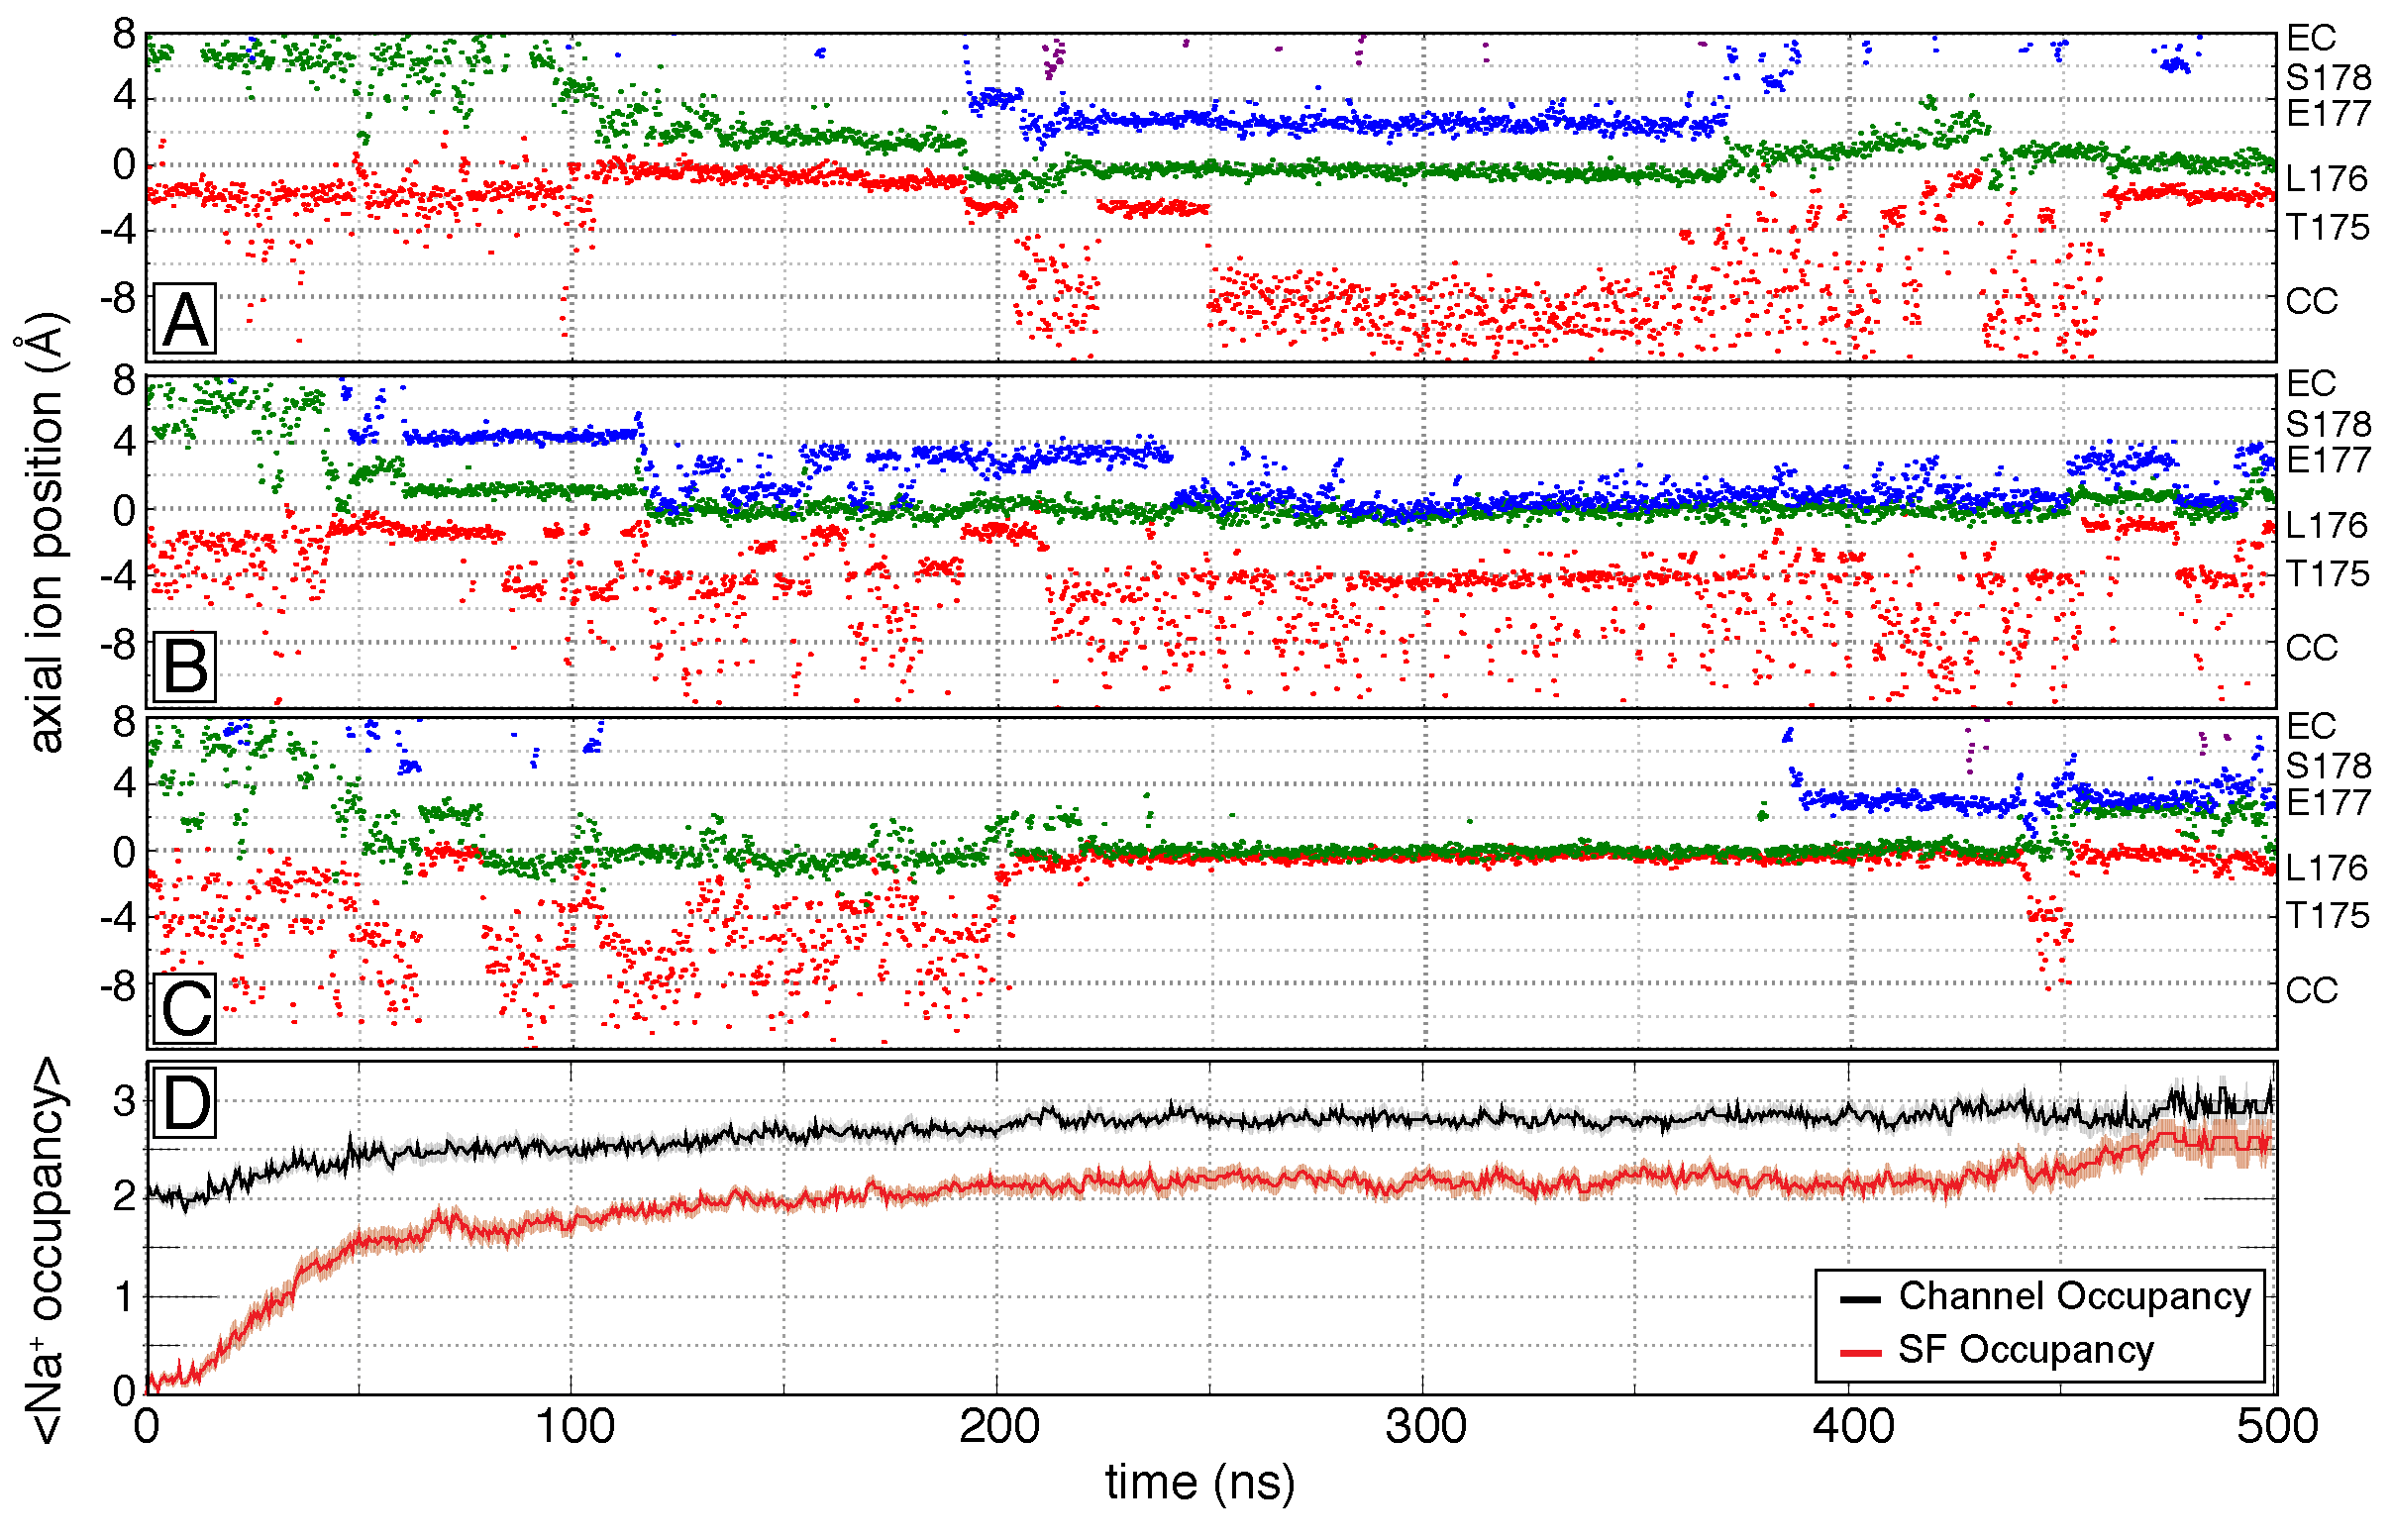
\includegraphics[width=0.9\textwidth]{navreview/revfig2}
\caption[Time series of axial Na$^{+}$ positions and average occupancy from unbiased equilibrium simulations of NavAb]{\textbf{Time series of axial Na$^{+}$ positions and average occupancy from unbiased equilibrium simulations of NavAb} (Chakrabarti et al. 2013). (\textbf{A-C}) Three out of forty-seven simulation repeats, where Na$^{+}$ reversibly diffuse in and out of the SF.  Na$^{+}$ cations are colored by depth rank within the SF from intracellular to extracellular (ordered red, green, blue in color, or lightest to darkest in grayscale).  The channel was initially devoid of cations and simulations differed in initial random velocities. (\textbf{D}) Time dependence of average Na$^{+}$ occupancy across all forty-seven simulation repeats for the channel (black, defined as any Na$^{+}$ within axial range 8 $\angstrom$ to -12 $\angstrom$) and SF (red, defined as any Na$^{+}$ with first-shell coordination to channel ligands E177 and L176).  Error bars are computed using the standard error of mean across all simulation repeats.  The simulation length of individual repeats varied from 450 to 500 ns, resulting in a smaller data set and increased noise in the last 50 ns of this time series.}
\label{fig:rev2}
\end{figure}

Although biased-sampling methods have been used to quantify the favorable binding sites of Na$^{+}$ and K$^{+}$ in the Nav channel SF, extensive unbiased equilibrium simulations have not been performed in the study of ionic selectivity.  In the field-strength model of K$^{+}$ selectivity by Noskov et al., it was suggested that the number and the type of ligands could directly influence selectivity \cite{Noskov:2006fd,Noskov:2004tv}. This model is interesting when viewed in the context of Nav channels, since conformational isomerization of E177 side chains may result in a variable number of coordinating ligands.  Chakrabarti et al. observe an average SF occupancy of $2.09 \pm 0.05$ Na$^{+}$ cations coordinated by an average of $2.23 \pm 0.04$ carboxylate groups, whereas the average SF occupancy of K$^{+}$ and its average coordinate to carboxylate side chains is yet to be determined \cite{Chakrabarti:2013kd}.  Simulations by Ngo et al. suggest that carboxylate coordination contributes to K$^{+}$ blockage during inward conduction, but they did not explicitly study the effect of conformational isomerization with respect to selectivity of Na$^{+}$ \cite{Ngo:2016es}.  Using biomimetic graphene pores containing carboxylate or carbonyl groups, He et al. studied the voltage dependence of Na$^{+}$ and K$^{+}$ currents as well as selectivity \cite{He:2013it}.  A graphene pore with three carboxylate groups was found to be Na$^{+}$-selective at low voltage and K$^{+}$-selective at high voltage in mixed-cation solutions.  Voltage was also found to induce conformational changes in carboxylate group orientation with respect to the direction of the electric field, with an out-facing state associated with K$^{+}$ selectivity and and lumen-facing state associated with Na$^{+}$ selectivity.  While there are many differences between such simplified models and the complex environment of the SF of Nav channels, this study supports a putative mechanism of selectivity involving the conformational isomerization of E177 side chains that remains to be examined in Nav channels.
 
 In Nav channels, multi-microsecond simulations have yet to be used to study the selectivity of Na$^{+}$ over Ca$^{2+}$. In addition to long simulation timescales, polarizable force fields may be required to reach quantitative estimates of Na$^{+}$:Ca$^{2+}$ conductance ratios that match experimental values.  Because the ionic radii of Na$^{+}$ and Ca$^{2+}$ are very similar (1.16 \angstrom and 1.14 \angstrom, respectively), an accurate treatment of Ca$^{2+}$ requires the use force fields that account for electronic polarization in the environment surrounding the ion, since the valence charge is greater for Ca$^{2+}$ \cite{Huang:2014ia}. Non-polarizable models of Ca$^{2+}$ fail to reproduce protein-ion binding energies from using quantum mechanical calculations over a diverse range of cation binding sites \cite{Ngo:2015ki}. It has been shown that electronic polarization results in significant ion-induced dipole shifts on the carbonyl groups of the SF in KcsA \cite{Allen:2006jw,Bucher:2009ef}, but this effect is unknown in Nav channels.  As such, quantitative estimates from Nav channel simulations of Ca$^{2+}$ using non-polarizable force fields must be considered carefully.
 
 \section{Perspectives}
 Computational studies of bacterial Nav channels offer a unique perspective on molecular mechanisms of ionic permeation in a weakly-selective channel.  The consensus mechanism of Na$^{+}$ permeation consists of a weakly-coupled knock-on involving approximately two ions on average.  Multiple studies have described the lowest-energy, two-ion occupancy state of the SF as one in which ions are partially dehydrated and bind the SF in off-axis fashion in an upper site (S$_{HFS}$) and a lower site (S$_{CEN}$ and/or S$_{IN}$).  Permeation occurs via these two sites with low ($\sim$1-2 kcal/mol) intervening free energy barriers and the cations are able to pass one another, with occasional double occupancy of one or more sites in the SF.  Although no consensus model of Na$^{+}$ selectivity has yet been established, several proposed mechanisms attribute selectivity to high permeation barriers between upper and lower binding sites for K$^{+}$ and Ca$^{2+}$.  
In qualitative agreement with experiment, most of the simulation studies of cation permeation in Nav channels published to this date support a rapid conduction process.  Equilibrium simulations of Na$^{+}$ in NavAb yielded estimates of permeation rates with the correct order of magnitude for a sodium channel \cite{Chakrabarti:2013kd}.  Estimates of Na$^{+}$ conductance computed from two non-equilibrium studies were in good agreement with experimental values \cite{Ke:2014fy,Ulmschneider:2013da}.  One of these studies also reported a Na$^{+}$:K$^{+}$ conductance ratio commensurate with experimental measurements, while all other studies of Na$^{+}$ selectivity over K$^{+}$ and Ca$^{2+}$ were qualitatively correct.  Future studies of ionic selectivity in Nav channels will benefit from more comprehensive sampling of different ionic species in order to assess the importance of conformational isomerization of Glu side chains in this process.  In an effort to reproduce experimental selectivity ratios, it would be useful to conduct simulations of Nav channels in bi-ionic conditions in the presence of applied voltage to compute reversal potentials.
In order to obtain simulation results that are minimally biased by systematic and statistical error, we suggest performing multiple repeats of unbiased equilibrium simulations as the optimal approach.  Individual simulations should be long enough to observe SF conduction events (requiring computational resources accessible on non-specialized supercomputers), with improved sampling due to randomized initial velocities and positions that may sample more uncorrelated ion binding modes than single long-time simulations.  Equilibrium simulations (with 0 mV applied voltage) are a good approximation to the low physiological voltages associated ion conduction \cite{Hille:2001tw}, but non-equilibrium simulations may also be used in the limit of low applied voltage in the physiological regime.  When biased sampling approaches are utilized, accelerated sampling algorithms such as bias-exchange metadynamics offer some benefits over umbrella sampling \cite{Domene:2015kj}. However, even these approaches would benefit from multiple simulation repeats to ensure that infrequent structural transitions involving other degrees of freedom, such as conformational isomerization of E177 side chains, are appropriately sampled, failing which, reaction coordinates including channel degrees of freedom could be considered.
One important issue that must be considered in evaluating simulations is that they have been performed using different simulation methodologies (biased, unbiased equilibrium, and unbiased non-equilibrium sampling), different force fields (CHARMM, AMBER, OPLS), different channel structures (closed and open conformations), and different simulation conditions (such as temperature, ionic concentration, and applied voltage) (Tables \ref{table:biased}, \ref{table:unbiased}). For Na$^{+}$ channels, these differences result in discrepancies in estimates of ion binding, permeation, and selectivity.  Dataset sizes varied between 0.1 and 10 microseconds of aggregate sampling between studies, and as such, it is not realistic to expect a consensus on the details of permeation and selectivity.  In general, continued progress in computer simulation studies of ion channels will greatly benefit from the quantification of both systematic and statistical errors. 
 
 
\printbibliography[heading=subbibnumbered,title={References}]
 \end{refsection}